\section{Concurrency and Data Scheduling Abstractions}
\label{sec:concurrency_abstractions}

Concurrency and data scheduling abstractions rely heavily on language semantics. In this section we explore semantics of three distinctively different languages: C++\footnote{C++ is required because reference \code{\&} variables are not available in C. More advanced C++ capabilities are not always synthesizable, thus rarely used for hardware description.}, VHDL, and DFiant.

Consider a function $f$ and its implementations, as detailed in Table \ref{tbl:DataSchedDefImpl}. Despite similar code appearance, the semantics are very different, as depicted in Fig. \ref{fig:DataSchedGraph}. The following subsections qualify these semantics.


%\setlength{\belowcaptionskip}{-15pt}
\begin{figure}[t]
    \vspace*{-6ex}
  \centering
  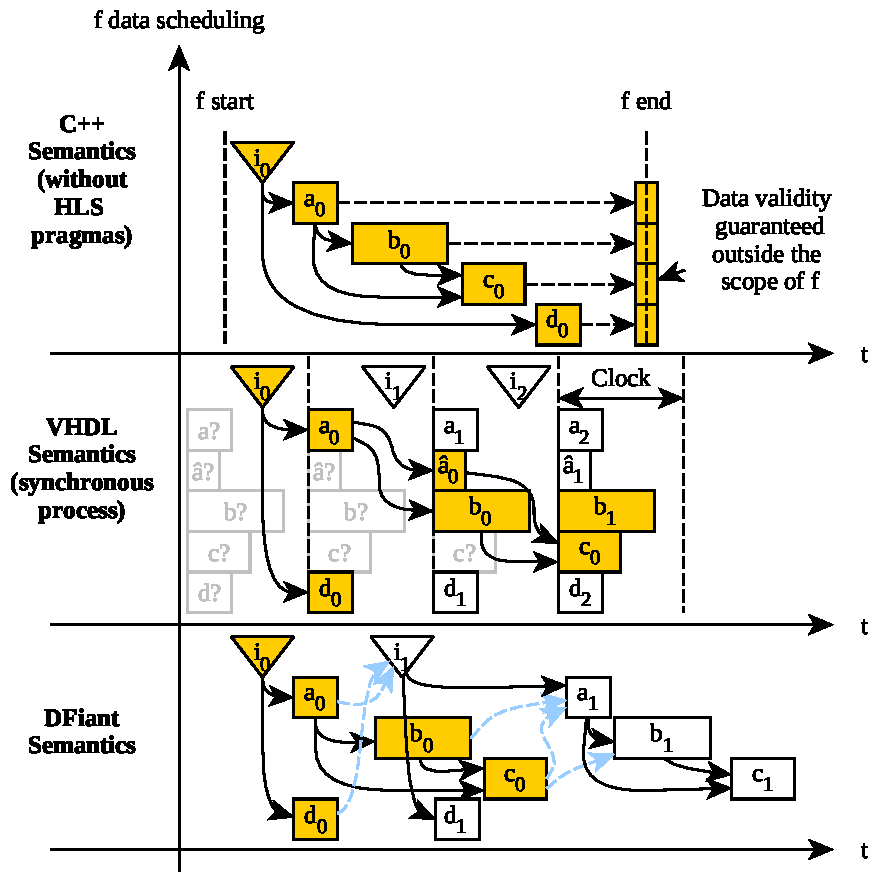
\includegraphics[width=\linewidth]{graphics/DataScheduling.pdf}
  \captionof{figure}{$f$ data scheduling semantics in C++, VHDL, and DFiant}
  \label{fig:DataSchedGraph}
\end{figure}


\subsection{C++ Semantics}
Sequential programming models, such as C++, do not possess concurrent semantics that allow the independent parts of \code{f} to run concurrently. Data scheduling order is set by the \textit{code statement order} and cannot be pipelined. \code{f} can be executed in parallel by more than one thread, but each thread runs \code{f} sequentially and as a whole\footnote{We only observe language semantics. Out-of-order or multi-processor executions may still apply.}. These concurrent semantics are important both for fine-grain parallelism and flexible concurrent code composition, as we demonstrate later in Section~\ref{sec:type_system}.  HLS utilities extend sequential languages with \code{pragma} directives that change semantics. We observe the C++ \code{f} implementation as follows:


\begin{enumerate}[leftmargin=*]
  \item All statements are variable assignments.
  \item \code{d} is independent of \code{a}, \code{b}, and \code{c} but cannot be scheduled concurrently. Additionally, \code{a} cannot be safely read until \code{f} finishes. Proper pragmas allow dataflow analysis and function inlining to overcome these limitations.
  \item Time between/of the data operations is unconstrained. The code does not restrict the functional requirement and will maintain correctness for every hardware synthesis fitting its semantics. 
\end{enumerate}  

\subsection{VHDL Semantics}
The RTL programming model is concurrent. Data scheduling is manual and clock-bound, while the order is set by the \textit{assignment cycle-time}. VHDL process semantics are different for \textit{signals} and \textit{variables}: signals are updated when the process ends, while variables are updated instantly. When embedded in a signal edge-detection conditional construct, both signals and variables can be interpreted as registers, depending on the context. We observe the VHDL \code{f} implementation as follows:

\begin{enumerate}[leftmargin=*]
  \item All statements are synchronous signal assignments with an explicit single-clock dependency. Clocked \code{f} imposes time restrictions to $f$. Although this implementation does not contradict the formal definition of $f$, its correctness is guaranteed solely under these restrictions.
  \item A latency balancing register added to maintain correctness of the \code{c} assignment pipeline\footnote{We can use VHDL variable to avoid latency balancing, by forming a combinational circuit.}. 
  \item Data is scheduled for every clock cycle, thus creating a pipeline. Each output signal is valid at a different time. Invalid outputs may be accessed, since VHDL has no implicit $guard$ semantics. More hardware is required to match the output cycle-latencies, and implement explicit guards.
  \item The implementation is very fragile and has limited reusability. Foremost, VHDL process construct alone is not reusable and requires an \textit{entity-architecture} encapsulation for structural instantiation. Additionally, \code{f} is tightly-coupled to \code{clk} timing and logic propagation delay. The slightest change in requirements or target device can lead to a painful redesign. 
\end{enumerate}

\subsection{DFiant Semantics}
DFiant has a dataflow programming model. Data scheduling order, or \textit{token-flow}, is set by the \textit{data dependency}. Essentially, the DFiant semantics schedules all independent dataflow expressions concurrently, while dependent operations are synthesized into a guarded FIFO-styled pipeline. Dataflow branches are implicitly forked and joined. Semantically, unused nodes, always consume tokens and are discarded during compilation. We observe the DFiant \code{f} implementation as follows:

\begin{enumerate}[leftmargin=*]
  \item All expressions are dataflow variable declarations.
  \item Concurrency is implicit. Function \code{f} is coded intuitively in a sequential manner, since dataflow dependencies are oblivious to statement order. 
  \item Data scheduling is implicitly guarded by data dependencies. For example, \code{a} is forked into both \code{b} and \code{c} operations, while \code{c} joins branches from \code{a} and \code{b}.
  It is impossible to read an invalid result or an old result (without extending semantics further).
  \item DFiant semantics are intuitive: data is consumed only when it is ready and can be accepted by all receiving nodes, while back-pressure prevents data loss. 
  \item A literal value (e.g., \code{5}) is a token generator that can produce infinite tokens (its production rate is set by the consumer).
\end{enumerate} 
   

\subsection{Comparing Semantics}
When comparing DFiant and VHDL, it is evident that DFiant is less verbose and has better semantics for code reuse. The DFiant compiler generates a hardware description that respects the design, timing, and target device constraints, in contrast to the given VHDL implementation which is equivalent to a singular possible DFiant code compilation for a given set of constraints.
DFiant prevents \code{f} users from reading invalid values, while in VHDL it must be programmed explicitly. Bluespec and Chisel have similar semantics to VHDL, thus suffer from related limitations (e.g., explicit pipelining). Fortunately, they both can provide guarded types that prevent invalid data use.

When comparing DFiant and C++, we observe that C++ HLS tools rely on code analysis and pragma directives to change the semantics of their sequential code, while DFiant has its own dataflow type system that guarantees its seamless concurrent semantics. Consequently, C++ HLS tools limit language constructs and hierarchies which are not supported by the analysis algorithms (e.g., recursion), in contrary to DFiant which supports all finite Scala constructs (e.g., finite generation loops and recursions). 
%We believe that constraint directives should not change semantics but refine them.

Contrarily, tandem operations are described more naturally in C++, and loops are utilized to describe repetitive dependent tasks. With proper pragmas, C++ loop iterations can run concurrently, but since they can also run sequentially, loops, and nested loops especially, may be semantically confusing. For this reason, DFiant does not support loops, same as VHDL (hardware generation loops are supported), and opts for state machine semantics to describe sequential operations. %We cover state in the next section. 
%We further compare DFiant against other HLS tools and languages in Section \ref{sec:related_work}. 
